\documentclass{article}

\usepackage{graphicx}

\usepackage{placeins}%Eklenen resim ve figürlerin bulundukları bölümde sabit kalmaları için
\usepackage{blindtext}
\usepackage{bredzenie}

\author{John Surname}
\date{\today}
\title{My Document with Picture}

\begin{document}
\maketitle

\part{Part Title}

\blindtext

\bredzenie{2}

\blindtext
\section{Section Title}

\blindtext
\begin{figure}[t]
  \centering
  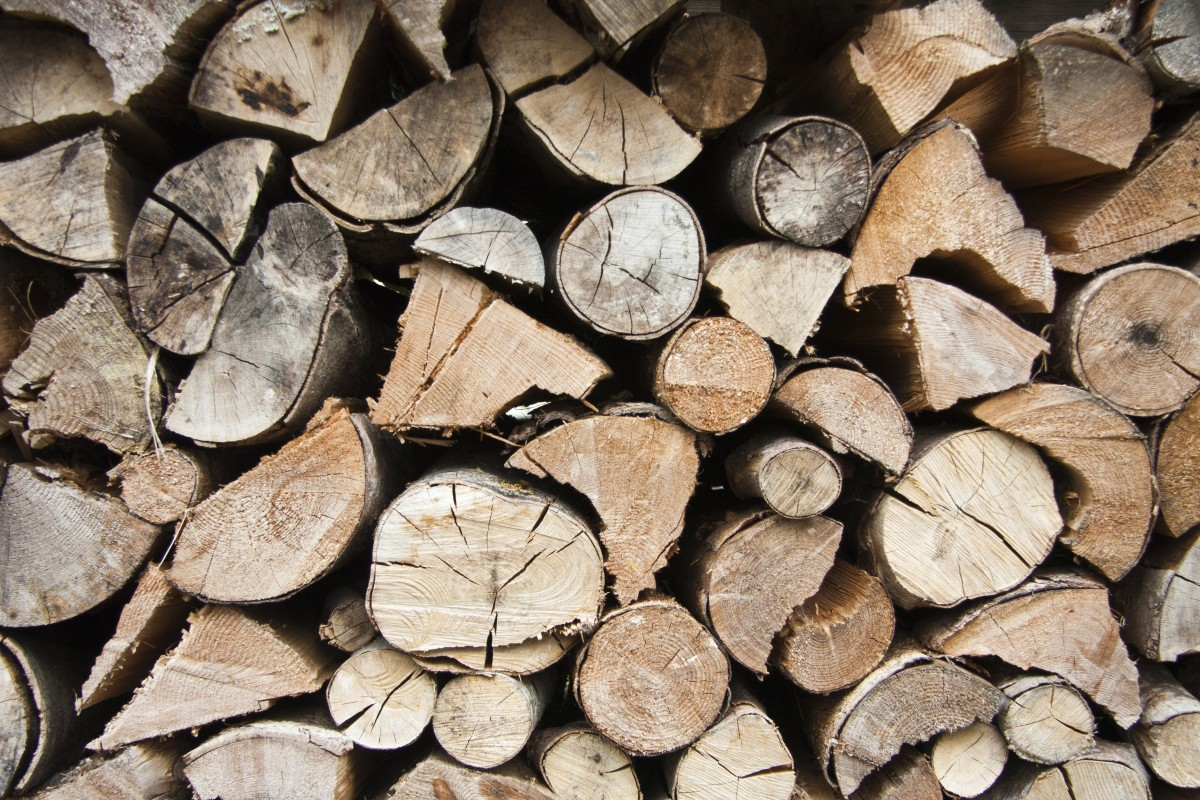
\includegraphics[scale=1.0]{eximg01.jpeg}
  \caption{My Figure Full Scale}
  \label{fig:My Fig Full}
\end{figure}

\FloatBarrier

\bredzenie{2}

\begin{figure}[t]
  \centering
  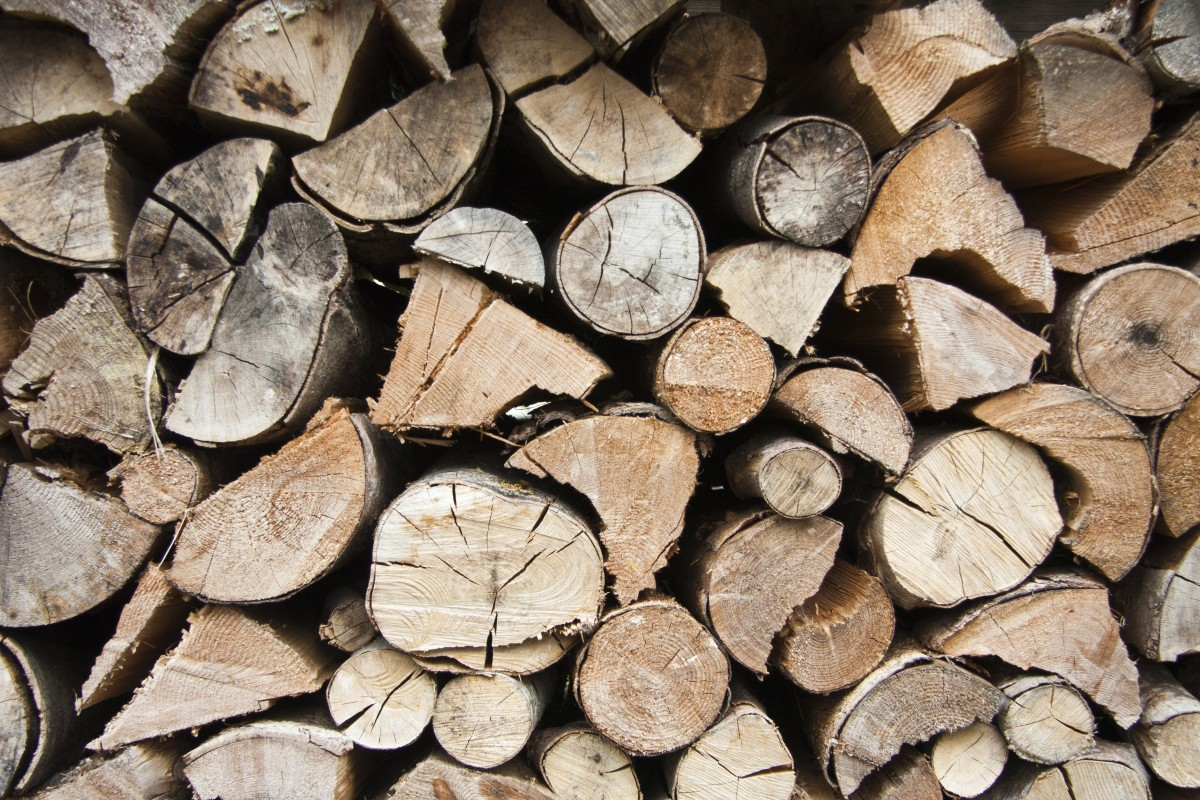
\includegraphics[width=\textwidth, keepaspectratio]{eximg01.jpeg}
  \caption{My Figure Fit to Textwidth with aspect ratio}
  \label{fig:My Fig Full}
\end{figure}


\bredzenie{2}

\subsection{Subsection Title}

\blindtext
\begin{figure}[t]
  \centering
  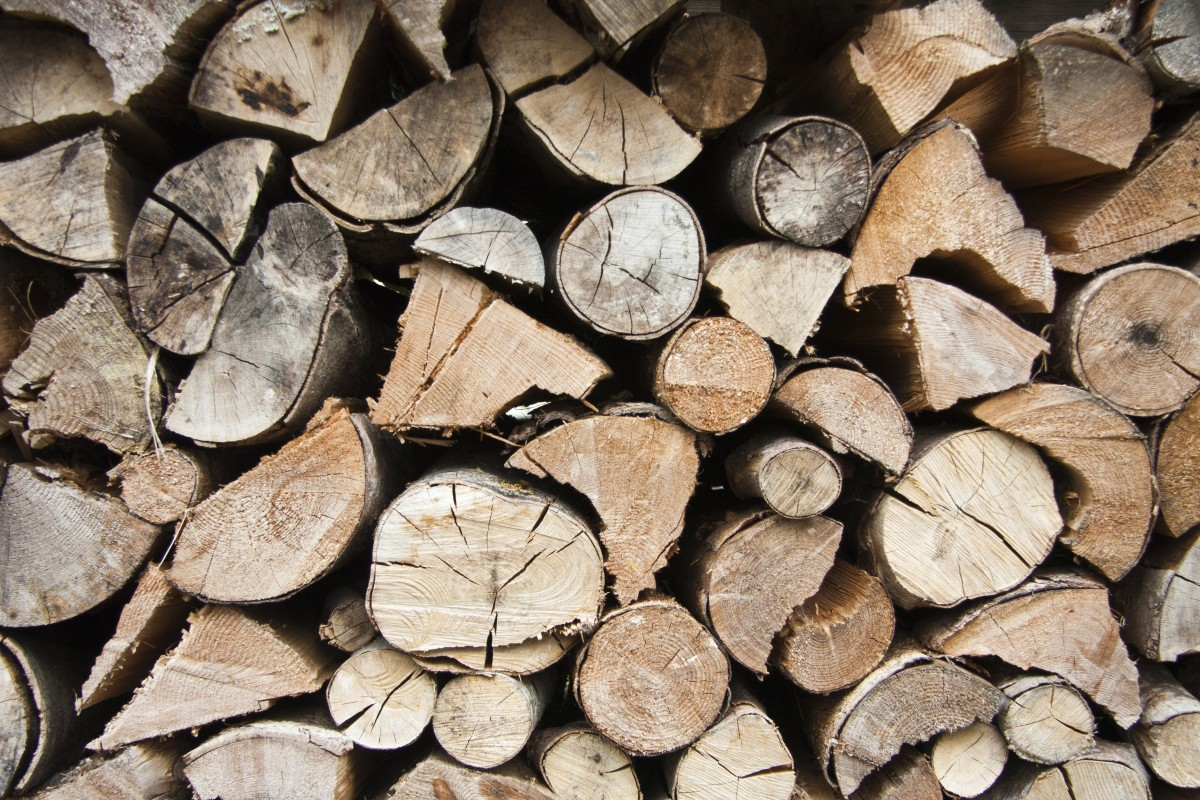
\includegraphics[scale=0.5]{eximg01.jpeg}
  \caption{My Figure Half Scale}
  \label{fig:My Fig Half}
\end{figure}
\FloatBarrier

\bredzenie{1}

\blindtext
\begin{figure}[t]
  \centering
  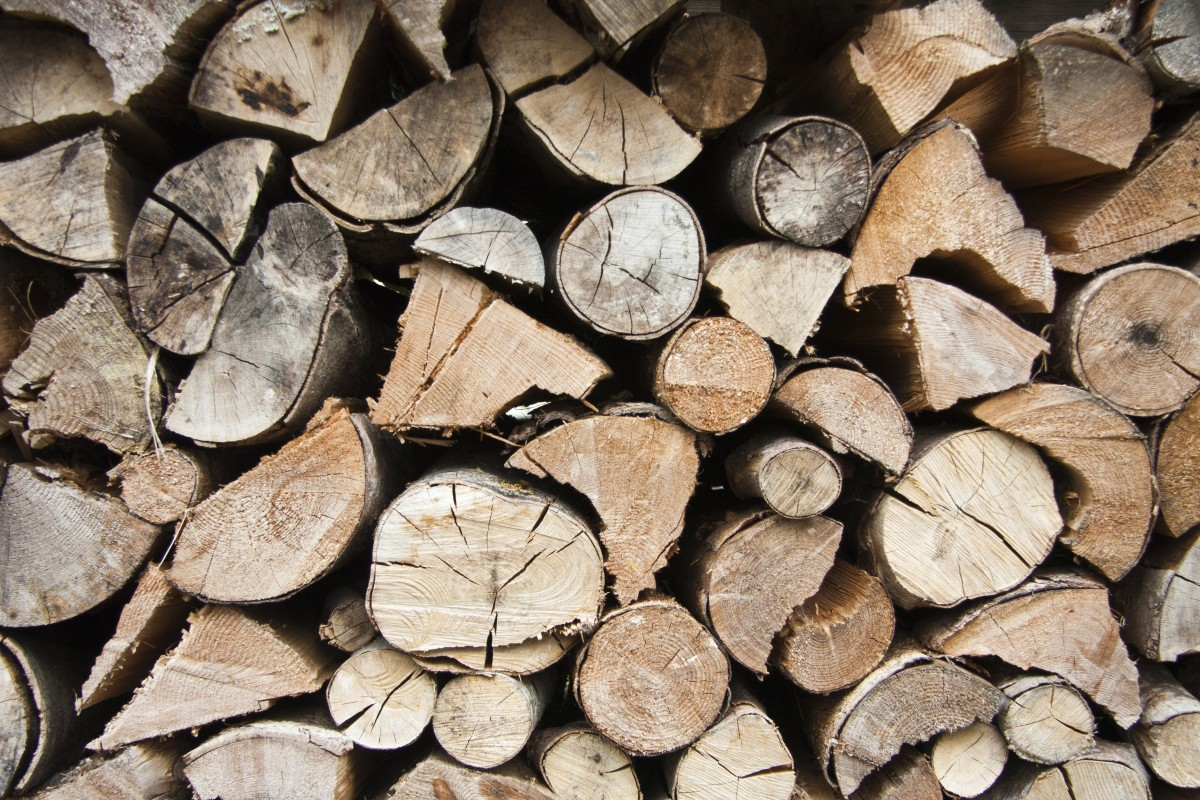
\includegraphics[scale=0.3]{eximg01.jpeg}
  \caption{My Figure 1/3 scale}
  \label{fig:My Fig Half}
\end{figure}
\FloatBarrier

\bredzenie{2}

\end{document}